% !TEX root = main.tex

\section{凸函数} % 3.5
\subsection{基本概念与性质}
\begin{definition}[凸函数]
	凸函数的几种基本定义如下
\begin{enumerate}
	\item 原始定义:$f:\rn\to\rr$为凸$\iff\dom f$为凸,且
\[\forall \vx,\vy\in\dom f,\theta\in[0,1]:\;f(\theta \vx+(1-\theta)\vy)\leq\theta f(\vx)+(1-\theta)f(\vy)\]
\begin{itemize}
	\item 严格凸:$\theta\in(0,1)$,不等式不能取等
	\item 凹函数:若$-f$为凸
\end{itemize}
	\item 高维定义:
$f:\rn\mapsto\rr$为凸$\iff\dom f$为凸,且
\[\forall \vx\in\dom f,\vv\in\rn:g(t):=f(\vx+t\vv)\text{为凸,}\dom g=\{t\mid \vx+t\vv\in\dom f\}\]
相当于每一个剖面上的低维函数都是凸的(固定$\vx$和$\vv$变化$t$看凸性,则$\vx+t\vv$在一条直线上/超平面上移动)
	\item 一阶条件(first-order condition)\footnote{$\nabla^\T f(\vx)=[\nabla f(\vx)]^\T$, $\nabla^2 f(\vx)$为$f(\vx)$的Hessian矩阵,其他关于矩阵微积分的知识请见附录\ref{appendix:matrix}节}:$f:\rn\mapsto\rr$为凸$\iff\dom f$为凸,且
	\[f(\vy)\geq f(\vx)+\nabla^\T f(\vx)(\vy-\vx)\]
	即Taylor公式一阶展开
	\begin{analysis}
		用高维定义证明,先证一维情况,然后设$g(t)=f(t\vy+(1-t)\vx)$,并对$t$求导。
		由于$g(t)$是凸的,故用一维情况得证
	\end{analysis}
	\item 二阶条件:% 3.7
	$f:\rn\mapsto\rr$为凸$\iff\dom f$为凸,且
	\[\forall \vx\in\dom f:\nabla^2 f(\vx) \succeq 0\]
	\begin{itemize}
		\item 凹函数:$\nabla^2 f(\vx)\preceq 0$
		\item 严格凸:\textcolor{red}{$\impliedby$}$\nabla^2 f(\vx)\succ 0$,反例$f(x)=x^4$(在一个点斜率不变并不要紧)
	\end{itemize}
	\begin{analysis}
		同样先证明一维情况,然后设$g(t)=f(\vx+t\vv)$,并对$t$求二阶导,类似可得证
	\end{analysis}
\end{enumerate}
\end{definition}

\begin{example}
$f(\vx)=\va^\T \vx+\vb$
\end{example}
\begin{analysis}
有$\nabla f(\vx)=\va$,进而
\[f(\vy)=\va^\T \vy+\vb\geq \va^\T \vx+\vb+\va^\T(\vy-\vx)=\va^\T \vy+\vb\]
\end{analysis}

\begin{example}
	假设$f:\rr\mapsto\rr$为凸函数,$a<b$
	\begin{enumerate}
		\item $\disp\forall x\in[a,b]:\;f(x)\leq\frac{b-x}{b-a}f(a)+\frac{x-a}{b-a}f(b)$\\
		由$f(\theta a+(1-\theta)b)\leq \theta f(a)+(1-\theta)f(b)$,令
		\[\theta a+(1-\theta)b=x\implies\theta=\frac{x-b}{a-b}\]
		代入得证
		\item $\disp\forall x\in[a,b]:\;\frac{f(x)-f(a)}{x-a}\leq\frac{f(b)-f(a)}{b-a}\leq\frac{f(b)-f(x)}{b-x}$\\
		展开等价于(1)式
		\item 假设$f$可微,
		\[f'(a)\leq \frac{f(b)-f(a)}{b-a}\leq f'(b)\]
		由(2)式取极限可得
		\item 假设$f$二次可微,有$f''(a)\geq 0$以及$f''(b)\geq 0$\\
		令$b=x$,由(3)式,$f'(x)-f'(a)\geq 0\implies f''(a)\geq 0$
	\end{enumerate}
\end{example}

\begin{definition}[凸函数的扩展(extended-value)]
尽管凸函数的定义域为凸,但往往不好处理,那就将其扩展到全空间。
$\vx\in\dom f\subset\rn, \dom\widetilde{f}=\rn$,会有
\[\widetilde{f}(\vx)=\begin{cases}f(\vx)&\vx\in\dom f\\+\infty&\vx\notin\dom f\end{cases}\]
\end{definition}
\begin{example}[示性(indicator)函数]
	扩展值延伸的示性函数是凸的
\[\tilde{I}_\sC(\vx)=\begin{cases}0&\vx\in \sC\\ +\infty & \vx\notin \sC\end{cases}\]
\end{example}

\begin{theorem}
若$f$为凸,可微,则$\exists \vx\in\dom f,\nabla f(\vx)=0$
\end{theorem}

\begin{example}
二次函数$f(\vx)=\dfrac{1}{2}\vx^\T P\vx+\vq^\T \vx+r$,$P\in \bbs^n$(对称矩阵),$\vq\in\rn$,$r\in\rr$
\end{example}
\begin{analysis}
$\nabla f(\vx)=\frac{1}{2}(P+P^\T)\vx+\vq\implies\nabla^2 f(\vx)=P$\\
故$P\in \bbs^n_+$,$f(\vx)$为凸;$P\in \bbs_{++}^n$,$f(\vx)$严格凸
\end{analysis}

\begin{example}
$f(x)=\dfrac{1}{x^2},\;\dom f=\lrb{x\in\rr,x\ne 0}$
\end{example}
\begin{analysis}
注意$\dom f$不是凸集
\end{analysis}

\subsection{常见例子}
\subsubsection{$\rr$上的函数}
\begin{itemize}
	\item 仿射函数$f(x)=ax+b$
	\item 指数函数$f(x)=\ee^{ax}$
	\item 幂函数$f(x)=x^a$
	\item 绝对值的幂函数$f(x)=|x|^p,x\in\rr,p>0$:$p\in[1,+\infty)$凸,$p\in(0,1)$既不凸又不凹
	\begin{analysis}
	\[f''(x)=\begin{cases}
	p(p-1)x^{p-2} & x<0\\
	p(p-1)(-x)^{p-2} & x<0
	\end{cases}\]
	\end{analysis}
	\item 对数函数$f(x)=\log x$
	\item 熵$f(x)=-x\log x$
\end{itemize}

\subsubsection{$\rn$上的函数}
\begin{itemize}
	\item 任意范数$f(\vx)=\norm{\vx}$(常被用来\textbf{正则化}!)
\begin{analysis}
	由三角不等式
\[\forall \vx,\vy,\theta\in[0,1]:\;
\norm{\theta \vx+(1-\theta)\vy}\leq \norm{\theta \vx}+\norm{(1-\theta)\vy}\leq \theta \norm{x}+(1-\theta)\norm{y}\]
\end{analysis}
	\item 极大值函数$f(\vx)=\max\lrb{x_1,\ldots,x_n},x\in\rn$
\begin{analysis}
	由原式定义
	\[f(\theta\vx+(1-\theta)\vy)=\max_i(\theta x_i+(1-\theta)y_i)\leq\theta\max_i x_i+(1-\theta)\max_i y_i=\theta f(\vx)+(1-\theta)f(\vy)\]
\end{analysis}
	\item 二次线性分式函数$f(\vx,y)=x^2/y,(x,y)\in\rr^2,y>0$
\begin{analysis}
	由二阶条件
	\[\nabla^2f(\vx,y)=\frac{2}{y^3}\bmat{y^2 & -xy\\-xy & x^2}=\frac{2}{y^3}\bmat{y\\-x}\bmat{y\\-x}^\T\succeq 0\]
\end{analysis}
	\item 指数和的对数$f(\vx)=\log(\ee^{x_1}+\cdots+\ee^{x_n})$
\begin{analysis}
此即极大值函数的解析近似\footnote{即无穷阶可微},因有下式成立
\[\max\{x_1,\ldots,x_n\}\leq f(\vx)\leq\max\{x_1,\ldots,x_n\}+\log n\]
利用二阶条件证明凸性
\[\begin{aligned}
\pd{f}{x_i}&=\frac{\ee^{x_i}}{\ee^{x_1}+\cdots+\ee^{x_n}}\\
\pddxy{f}{x_i}{x_j}&=
\begin{cases}
\frac{-\ee^{x_i}\ee^{x_j}}{(\ee^{x_1}+\cdots+\ee^{x_n})^2} & i\ne j\\
\frac{\ee^{x_i}(\ee^{x_1}+\cdots+\ee^{x_{i-1}}+\ee^{x_{i+1}}+\cdots+\ee^{x_n})}{(\ee^{x_1}+\cdots+\ee^{x_n})^2} & i=j
\end{cases}
\end{aligned}\]
\[\vz:=\bmat{\ee^{x_1}&\cdots&\ee^{x_n}}^\T\]
求Hessian矩阵
\[\nabla^2f(\vx)=\frac{1}{(\vone^\T \vz)^2}((\vone^\T \vz)\opdiag(\vz)-\vz \vz^\T)\]
将前面常量丢弃
\[\begin{aligned}
\vv^\T \nabla^2f(\vx)\vv&=(\mathbbm{1}^\T \vz)\vv^\T \opdiag(\vz)\vv-\vv^\T \vz\vz^\T \vv\\
&=\lrp{\sum_i z_i}\lrp{\sum_i v_i^2 z_i}-\lrp{\sum_i v_i z_i}^2\\
&\qquad\mbox{令$\va_i:=\vv_i\sqrt{\vz_i}=\bmat{a_1&\cdots&a_n}^\T,b_i:=\sqrt{\vz_i}$}\\
&=(\vb^\T \vb)(\va^\T \va)-(\va^\T \vb)^2\qquad\text{Cauchy}\\
&\geq 0
\end{aligned}\]
进而$\nabla^2f(\vx)$半正定,即$\nabla^2f(\vx)\succeq 0$
\end{analysis}
	\item 几何平均$f(\vx)=\disp \lrp{\prod_{i=1}^n x_i}^{1/n}$为凹函数
\begin{analysis}
	\[\pddxy{f}{x_k}{x_l}=\begin{cases}
		-(n-1)\frac{\lrp{\prod_{i=1}^n x_i}^{1/n}}{n^2x_k^2} & k=l\\
		\frac{\lrp{\prod_{i=1}^n x_i}^{1/n}}{n^2x_k x_l} & k\ne l
	\end{cases}\]
	进而
	\[\nabla^2 f(\vx)=-\frac{\lrp{\prod_{i=1}^n x_i}^{1/n}}{n^2}\lrp{n\sum_{i=1}^n \frac{v_i^2}{x_i^2}-\lrp{\sum_{i=1}^n\frac{v_i}{x_i}}^2}\leq 0\]
	同样由Cauchy不等式可证得
\end{analysis}
	\item 对数行列式$f(X)=\log\det(X),\dom f=\bbs_{++}^n$为凹函数
\begin{analysis}
用高维定义
\[\begin{aligned}
g(t)&:=f( Z+t V)\\
&=\log\det( Z+t V)\\
&=\log\det( Z^{1/2}(I+t Z^{-1/2} V Z^{-1/2}) Z^{1/2}),\quad  Z^{1/2}\in \bbs_{++}^n, Z^{1/2} Z^{1/2}= Z\\
&=\log\det( Z)+\log\det(I+t Z^{-1/2} V Z^{-1/2})\\
&=\log\det( Z)+\sum_{i=1}^n\log(1+t\lambda_i),\quad \lambda_i\text{为} Z^{-1/2} V Z^{-1/2}\text{的特征值}
\end{aligned}\]
因此下式成立
\[\begin{aligned}
g'(t)&=\sum_{i=1}^n\frac{\lambda_i}{1+t\lambda_i}\\
g''(t)&=\sum_{i=1}^n-\frac{\lambda_i^2}{(1+t\lambda_i)^2}\leq 0
\end{aligned}\]
补充证明:对对称阵进行特征值分解$t Z^{1/2} V Z^{1/2}=tQ\Lambda Q^\T$,对角阵$\Lambda$即为
$QQ^\T=I$,Q为酉矩阵
\[\begin{aligned}
	I+t Z^{-1/2} V Z^{-1/2}&=QQ^\T+tQ\Lambda Q^\T=Q(I+t\Lambda)Q^\T\\
	\log\det(I+t Z^{-1/2} V Z^{-1/2})&=\log\det(Q)+\log\det(I+t\Lambda)+\log\det(Q^\T)
\end{aligned}\]
\end{analysis}
\end{itemize}

\subsection{保凸运算}
\begin{itemize}
	\item 非负加权和$f_1,\ldots,f_m$为凸,定义域$\rn$
	\[f:=\sum_{i=1}^m w_if_i,w_i\geq 0\]
	\item 非负积分$f(x,y)$对$y\in A$均为凸($A$不一定为凸),$w(y)\geq 0$
	\[g(x):=\int_{y\in A}w(y)f(x,y)\diff y\]
	\item 仿射映射$f:\rn\mapsto\rr$为凸,$A\in\rr^{m\times n},\vb\in\rn$,$\dom g=\{\vx\mid A\vx+\vb\in\dom f\}$
	\[g(\vx):=f(A\vx+\vb)\]
	\begin{analysis}
		$\dom f$为凸,则$\dom g$为凸
		\[\begin{aligned}
			\forall \vx,\vy\in\dom g,\forall\theta\in[0,1]:\;
		g(\theta \vx+(1-\theta)\vy)&=f(A(\theta \vx+(1-\theta)\vy)+\vb)\\
		&=f(\theta(A\vx+\vb)+(1-\theta)(A\vy+\vb))\\
		&\leq\theta f(A\vx+\vb)+(1-\theta)f(A\vy+\vb)\\
		&=\theta g(\vx)+(1-\theta)g(\vy)
		\end{aligned}\]
		其实只是在定义域上改变,而不是改变值域,因而函数凸性不会改变
	\end{analysis}

	\item 两个函数的极大值函数/逐点(pointwise)最大函数,$f_1,f_2$为凸
	\[f(x):=\max\{f_1(x),f_2(x)\},\dom f=\dom f_1\cap\dom f_2\]
	\begin{example}
	$\vx\in\rn$,$x[i]$为第$i$大元素,$x[1]\geq x[2]\geq\cdots\geq x[r]\geq\cdots\geq x[n]$
	\[f(\vx):=\sum_{i=1}^r x[i]\]
	\begin{itemize}
	\item[*] $r=1$:$f(\vx)=x[1]=\max\{x_1,\ldots,x_n\}$,每一项都是$\ee_i^\T x_i$
	\item[*] $r>1$:$f(\vx)=\max\{x_{i_1}+\cdots+x_{i_r}\mid 1\leq i_1<i_2<\cdots<i_r\leq n\}$\\
	即从$\vx$的分量中选取$r$个分量进行求和的所有可能组合的最大值,即$n!/(r!(n-r)!)$个线性函数的逐点最大,故为凸
	\end{itemize}
	\end{example}
	\item 任意个凸函数极大值函数为凸(分片线性函数)
	\[f(x)=\max\{\va_1^\T \vx+\vb_1,\ldots,\va_m^\T+\vb_m\}\]
	\item 无限个凸函数,$y\in A$,$f(x,y)$对于$x$为凸,则$g(x)=\sup_{y\in A} f(x,y)$为凸
	\begin{example}
	点$\vx$到集合$\sC$的最远距离
	\[f(\vx)=\sup_{\vy\in A}\|x-y\|\]
	位移对于范数凸性不会有影响
	\end{example}

	\item 函数的组合:$h:\rr^k\mapsto\rr,g:\rn\mapsto\rr^k$
	\[f:=h\circ g:\rn\mapsto\rr\]
	\begin{analysis}
	先考虑$n=k=1,\dom g=\rn,\dom h=\rr^k,\dom f=\rr$,$h,g$二阶可微
	\[\begin{aligned}
	f'(\vx)&=h'(g(\vx))\cdot g'(\vx)\\
	f''(\vx)&=h''(g(\vx))(g'(\vx))^2+h'(g(\vx))g''(\vx)>0
	\end{aligned}\]
	即当满足以下任一条件时,$f(\vx)$为凸
	\begin{itemize}
		\item $g$为凸,$h$为凸且不降
		\item $g$为凹,$h$为凸且不增
		\item (若定义域非全空间)$g$为凸,$h$为凸,扩展值函数$\tilde{h}$不降
		\item (若定义域非全空间)$g$为凹,$h$为凸,$\tilde{h}$不增
	\end{itemize}
	\end{analysis}
	\begin{example}
	$g$为凸,$\exp g(\vx)$为凸;$g$为凹,$g>0$,$\log g(\vx)$为凹;$g$为凸,$g>0$,$1/g(\vx)$为凸
	\end{example}
	\begin{example}
	$g(\vx)=\vx^2,\dom g=\rr$,$h(y)=0,\dom h=[1,2]$,$f=h\circ g$,注意$\tilde{h}$并非不降!
	\end{example}

	\item 函数透视:$f:\rn\mapsto\rr,g:\rn\times\rr_{++}\mapsto\rr$
	\[g(\vx,t)=tf\lrp{\frac{\vx}{t}},\dom g=\lrb{(\vx,t)\mid\frac{\vx}{t}\in\dom f}\]
	若$f(\vx)$为凸,则$g(\vx,t)$相对于$(\vx,t)$联合凸
	\begin{analysis}
		考虑点$(\vx,t)$和$(\vy,s)$,有
		\[\begin{aligned}
		f\lrp{\frac{\theta\vx+(1-\theta)\vy}{\theta t+(1-\theta)s}}
		=&f\lrp{\frac{\theta t}{\theta t+(1-\theta)s}\frac{\vx}{t}+\frac{(1-\theta) s}{\theta t+(1-\theta)s}\frac{\vy}{s}}\\
		\leq&\frac{\theta t}{\theta t+(1-\theta)s}f\lrp{\frac{\vx}{t}}+\frac{(1-\theta) s}{\theta t+(1-\theta)s}f\lrp{\frac{\vy}{s}}
		\end{aligned}\]
	\end{analysis}
	\begin{example}
		考虑$\rr_{++}$上的凸函数$f(x)=-\log x$,其透视函数为
		\[g(x,t)=-t\log(x/t)=t\log(t/x)=t\log t-t\log x\]
		在$\rr_{++}^2$上为凸函数,称$g$为关于$t$和$x$的\textbf{相对熵}。
		\\进而可定义高维的相对熵$\vu,\vv\in\rr_{++}^n$
		\[g(\vu,\vv)=\sum_{i=1}^n u_i\log(u_i/v_i)\]
		由于是一系列$u_i,v_i$相对熵的和,故也是关于$(\vu,\vv)$的凸函数。
		\\另一方面可以定义$\vu,\vv\in\rr_{++}^n$之间的Kullback-Leibler/KL散度
		\[D_{KL}:=\sum_{i=1}^n\lrp{u_i\log\frac{u_i}{v_i}-u_i+v_i}\]
		由于是$(\vu,\vv)$相对熵和线性函数的和,因此也是凸函数
	\end{example}
	\begin{analysis}
		设
		\[f(\vu)=\sum_{i=1}^n u_i\log u_i \qquad (\nabla f(\vu))_i=\log u_i+1\]\
		由$f(\vu)$的凸性可得
		\[D_{KL}(\vu,\vv)=f(\vu)-f(\vv)-\nabla f(\vv)^\T(\vu-\vv)\geq 0\]
	\end{analysis}
\end{itemize}

\subsection{共轭函数}
\begin{definition}[函数的共轭(conjugate)]
	设函数$f:\rn\mapsto\rr,f^\star:\rn\mapsto\rr$
	\[f^\star(\vy)=\sup_{\vx\in\dom f}(\vy^\T \vx-f(\vx))\]
	几何意义即函数$f(\vx)$到不同斜率直线的垂直距离最大值,$\vy$可粗略理解为斜率,且$\vy^\T\vx$一定过原点
	\begin{figure}[H]
		\centering
		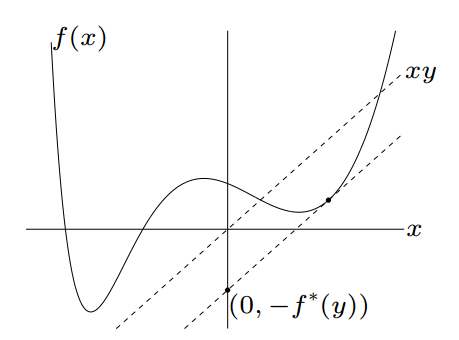
\includegraphics[width=0.4\linewidth]{fig/conjugate.PNG}
	\end{figure}
\end{definition}
由于$f^\star(\vx)$为一系列$\vy$的凸函数的逐点上确界,故$f^\star$为凸函数

\begin{example}
	一些共轭函数的例子如下
	\begin{itemize}
		\item 仿射函数:$f(x)=ax+b$,显然当斜率为$a$时(即平行),共轭函数才有界,故共轭函数定义域为单点集$\{a\}$,且$f^\star(a)=-b$
		\item 最大熵函数:$f(\vx)=\sum_{i=1}^nx_i\log x_i$
		\begin{analysis}
			按照定义进行拆分计算即可
			\[\begin{aligned}
				f^\star(\vy)&=\sup_\vx\sum_{i=1}^n x_i\log x_i\\
				&=\sum_{i=1}^n\sup_{x_i}y_i x_i-x_i\log x_i\qquad\mbox{求导可得}\\
				&=\sum_{i=1}^n\ee^{y_i-1}
			\end{aligned}\]
		\end{analysis}
	\end{itemize}
\end{example}

\subsection{拟凸函数}
\begin{definition}[$\alpha$次水平集($\alpha$-sub level set)]
$f:\rn\mapsto\rr$,$C_\alpha=\{\vx\in\dom f\mid f(\vx)\leq\alpha\}$
\end{definition}
\begin{definition}[拟凸函数(quasi-convex)]
所有$\alpha$次水平集为凸集$\iff$$f$为拟凸函数
\end{definition}
拟凸函数有很好的性质$\to$单模态/单峰函数
\begin{figure}[H]
	\centering
	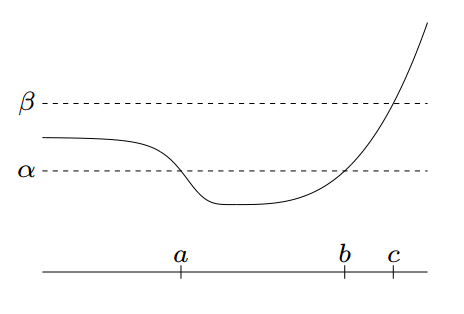
\includegraphics[width=0.4\linewidth]{fig/quasiconvex.PNG}
\end{figure}

\begin{theorem}
	可微拟凸函数判定条件
	\begin{itemize}
		\item 一阶条件:$\dom f$为凸集,且
		\[\forall \vx,\vy\in\dom f:\;f(\vy)\leq f(\vx)\implies\nabla f(\vx)^\T(\vy-\vx)\leq 0\]
		当$\nabla f(\vx)\ne 0$时,即$\nabla f(\vx)$在$\vx$处定义了水平集$\{\vy\mid f(\vy)\leq f(\vx)\}$的支撑超平面
		\begin{figure}[H]
			\centering
			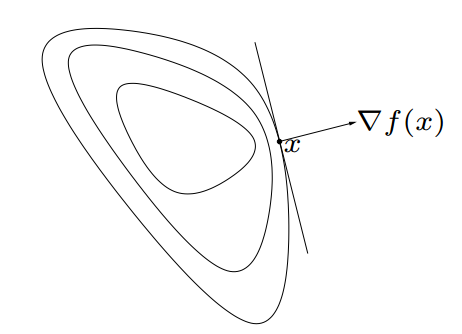
\includegraphics[width=0.4\linewidth]{fig/support-plane.PNG}
		\end{figure}
		\begin{analysis}
			同样考虑一维的情况,然后通过高维定义进行映射
		\end{analysis}
		\item 二阶条件:
		\[\forall \vx\in\dom f,\vy\in\rn:\;\vy^\T\nabla f(\vx)=0\implies \vy^\T\nabla^2f(\vx)\vy\geq 0\]
	\end{itemize}
\end{theorem}

\begin{example}[(拟)凸函数的判定]
	如下图,水平集显然凸(线段都在水平集内),故为拟凸函数,但对于直线\uppercase\expandafter{\romannumeral2},水平集间距离并不是越来越密,故不是凸函数
	\begin{figure}[H]
		\centering
		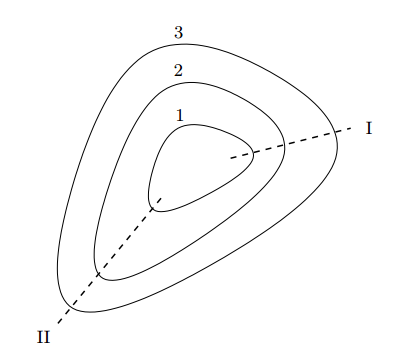
\includegraphics[width=0.35\linewidth]{fig/example-convex-function.PNG}
	\end{figure}
\end{example}

凸函数与凸集联系
\begin{itemize}
	\item 凸函数定义域为凸集,凸函数一定是拟凸函数
	\item 凸函数的$\alpha$次水平集为凸集
\end{itemize}